\chapter{Интеграл Римана и первообразная}\label{chap:c29}\markright{Глава 41}

\section{Площадь через нижние и верхние оценки}
\par\addvspace{5pt}\begin{lrbox}{\CatFlowBox}\begin{minipage}[t]{\linewidth}
\setlength{\parskip}{5pt}\setlength{\columnsep}{4.5mm}\setlength{\intextsep}{0pt}
\begin{wrapfigure}[11]{r}{54mm}

\includegraphics[width=54mm,height=58mm,keepaspectratio]{images/unique/art-120.png}
\label{catflow:120}
\end{wrapfigure}
Если скорость меняется со временем, произведение «скорость на время» приходится заменять суммой по коротким промежуткам. На каждом таком промежутке можно взять минимальную и максимальную скорость. Получаются две оценки общего перемещения. Если при измельчении сетки их можно сделать сколь угодно близкими, общий результат определяется однозначно. Так устроено определение интеграла.
\par\WFclear\end{minipage}\end{lrbox}%
\ifdim\dimexpr\ht\CatFlowBox+\dp\CatFlowBox\relax<64mm\dp\CatFlowBox=\dimexpr64mm-\ht\CatFlowBox\relax\fi%
\noindent\usebox{\CatFlowBox}\par\addvspace{5pt}
\begin{definition}
\term{Разбиение отрезка} (\emph{partition}) \([a;b]\), \(a<b\), — конечный набор точек \(P:\ a=x_0<x_1<\cdots<x_n=b\). Его \par \term{мелкость} (\emph{mesh}) равна \(\|P\|=\max_i(x_i-x_{i-1})\).
\end{definition}
\begin{definition}
Для ограниченной функции \(f:[a;b]\to\mathbb R\) \term{нижняя и верхняя суммы Дарбу} (\emph{lower and upper Darboux sums}) определяются формулами
\[
\begin{aligned}
m_i&=\inf_{x\in[x_{i-1};x_i]}f(x),&
M_i&=\sup_{x\in[x_{i-1};x_i]}f(x),\\
L(f,P)&=\sum_{i=1}^nm_i(x_i-x_{i-1}),&
U(f,P)&=\sum_{i=1}^nM_i(x_i-x_{i-1}).
\end{aligned}
\]
\end{definition}
\begin{theorem}[Измельчение разбиения]\label{thm:legacy-c29-1}
При добавлении точек разбиения нижняя сумма не уменьшается, верхняя не увеличивается. Для любых разбиений \(P,Q\) выполнено \(L(f,P)\le U(f,Q)\).
\end{theorem}
\begin{proof}
На меньшем отрезке инфимум не меньше прежнего, а супремум не больше прежнего. После умножения на длины частей и сложения получаем первое утверждение. Объединим точки \(P,Q\) в разбиение \(R\). Тогда \(L(f,P)\le L(f,R)\le U(f,R)\le U(f,Q)\).
\end{proof}
\begin{definition}
\term{Интегрируемость по Риману} (\emph{Riemann integrability}) ограниченной функции на \([a;b]\) означает равенство
\[
\sup_P L(f,P)=\inf_P U(f,P).
\]
Общее значение — \par \term{определённый интеграл} (\emph{definite integral}), обозначаемый \(\displaystyle\int_a^b f(x)\,dx\).
\end{definition}
\begin{theorem}[Критерий Дарбу; Darboux criterion]\label{thm:legacy-c29-2}
Ограниченная функция интегрируема тогда и только тогда, когда для любого \(\varepsilon>0\) существует разбиение \(P\) с \(U(f,P)-L(f,P)<\varepsilon\).
\end{theorem}
\begin{proof}
Обозначим нижний интеграл через \(I_-\), верхний через \(I_+\). По предыдущей теореме \(I_-\le I_+\). Если зазор сумм можно сделать меньше любого положительного числа, то \(0\le I_+-I_-\le U(f,P)-L(f,P)<\varepsilon\), значит, зазор интегралов равен нулю.
Если \(I_-=I_+=I\), из определений супремума и инфимума выберем \(P,Q\) с \(L(f,P)>I-\frac\varepsilon2\), \(U(f,Q)<I+\frac\varepsilon2\). Общее измельчение \(R\) имеет \(U(f,R)-L(f,R)<\varepsilon\).
\end{proof}
\begin{theorem}[Интегрируемость непрерывной функции]\label{thm:legacy-c29-3}
Непрерывная функция на отрезке интегрируема по Риману.
\end{theorem}
\begin{proof}
По главе \ref{chap:c28} функция ограничена и равномерно непрерывна. Выберем \(\delta>0\), при котором \(|x-y|<\delta\) влечёт \(|f(x)-f(y)|<\frac\varepsilon{b-a}\). Возьмём разбиение с мелкостью меньше \(\delta\). На каждой его части минимум и максимум достигаются, поэтому \(M_i-m_i<\frac\varepsilon{b-a}\). Тогда \(U-L=\sum_i(M_i-m_i)(x_i-x_{i-1})<\varepsilon\). Применяем критерий Дарбу.
\end{proof}
\begin{definition}
\term{Интегральная сумма Римана} (\emph{Riemann sum}) имеет вид \(S(f,P,\xi)=\sum_i f(\xi_i)(x_i-x_{i-1})\), где \(\xi_i\in[x_{i-1};x_i]\).
\end{definition}
\par\addvspace{5pt}\begin{lrbox}{\CatFlowBox}\begin{minipage}[t]{\linewidth}
\setlength{\parskip}{5pt}\setlength{\columnsep}{4.5mm}\setlength{\intextsep}{0pt}
\begin{wrapfigure}[11]{l}{54mm}

\includegraphics[width=54mm,height=58mm,keepaspectratio]{images/unique/art-121.png}
\label{catflow:121}
\end{wrapfigure}
Всегда \(L(f,P)\le S(f,P,\xi)\le U(f,P)\). Для непрерывной функции при \(\|P\|\to0\) верхняя и нижняя суммы сближаются по только что доказанной оценке; любая сумма Римана стремится к интегралу. Если функция принимает отрицательные значения, вклад соответствующих прямоугольников отрицателен. Для геометрической площади между графиком и осью нужно интегрировать \(|f|\).
\par\WFclear\end{minipage}\end{lrbox}%
\ifdim\dimexpr\ht\CatFlowBox+\dp\CatFlowBox\relax<64mm\dp\CatFlowBox=\dimexpr64mm-\ht\CatFlowBox\relax\fi%
\noindent\usebox{\CatFlowBox}\par\addvspace{5pt}
\section{Свойства определённого интеграла}
\begin{theorem}[Линейность, порядок и разбиение промежутка]\label{thm:legacy-c29-4}
Если \(f,g\) интегрируемы на \([a;b]\), а \(\alpha,\beta\in\mathbb R\), то
\[
\int_a^b(\alpha f+\beta g)\,dx
=\alpha\int_a^b f\,dx+\beta\int_a^b g\,dx.
\]
Из \(f\le g\) следует \(\int_a^b f\le\int_a^b g\). При \(a<c<b\) обе функции интегрируемы на частях отрезка и
\[
\int_a^b f(x)\,dx=\int_a^c f(x)\,dx+\int_c^b f(x)\,dx.
\]
\end{theorem}
\begin{proof}
Для общего разбиения сумма колебаний \(\alpha f+\beta g\), умноженных на длины частей, не превосходит \(|\alpha|(U_f-L_f)+|\beta|(U_g-L_g)\). Объединяя хорошие разбиения для \(f,g\), делаем эту величину сколь угодно малой. Критерий Дарбу доказывает интегрируемость линейной комбинации. На таких разбиениях каждая сумма Римана отличается от своего интеграла не больше соответствующего зазора \(U-L\). Линейность конечных сумм и стремление всех зазоров к нулю дают линейность интеграла.
Если \(f\le g\), то \(L(f,P)\le L(g,P)\) для каждого \(P\); взятие супремумов даёт порядок интегралов.
Добавим \(c\) в хорошее разбиение. Зазор сумм на каждой части не больше зазора на всём отрезке, поэтому обе части интегрируемы. Обратно, хорошие разбиения частей можно объединить. Нижние и верхние суммы на объединении равны суммам соответствующих величин на частях; при стремлении зазоров к нулю получаем аддитивность.
\end{proof}
Договоримся также, что \(\int_a^a f(x)\,dx=0\), а \(\int_b^a f(x)\,dx=-\int_a^b f(x)\,dx\). Это ориентированный интеграл: при перестановке пределов меняется знак.

\section{От производной к первообразной}
\begin{definition}
\term{Первообразная} (\emph{antiderivative}) функции \(f\) на интервале — дифференцируемая функция \(F\), для которой \(F'=f\). Если она определена и непрерывна на концах отрезка, производная на концах для последующих формул не требуется.
\end{definition}

\begin{definition}
\term{Неопределённый интеграл} (\emph{indefinite integral}) \(\int f(x)\,dx\) на интервале — семейство всех первообразных: \(F(x)+C\), где \(C\) — произвольная действительная постоянная. Любые две первообразные различаются на постоянную по теореме Лагранжа.
\end{definition}
\par\addvspace{5pt}\begin{lrbox}{\CatFlowBox}\begin{minipage}[t]{\linewidth}
\setlength{\parskip}{5pt}\setlength{\columnsep}{4.5mm}\setlength{\intextsep}{0pt}
\begin{wrapfigure}[11]{r}{54mm}

\includegraphics[width=54mm,height=58mm,keepaspectratio]{images/unique/art-122.png}
\label{catflow:122}
\end{wrapfigure}
Первообразная и определённый интеграл отвечают на разные вопросы. Первая восстанавливает функцию по её скорости изменения и оставляет произвольную постоянную. Второй вычисляет число, накопленное между двумя границами. Связь появляется у функции \(A(x)\), которая каждому верхнему пределу сопоставляет накопленный интеграл: при небольшом сдвиге границы добавляется узкая полоска площади.
\par\WFclear\end{minipage}\end{lrbox}%
\ifdim\dimexpr\ht\CatFlowBox+\dp\CatFlowBox\relax<64mm\dp\CatFlowBox=\dimexpr64mm-\ht\CatFlowBox\relax\fi%
\noindent\usebox{\CatFlowBox}\par\addvspace{5pt}
\begin{theorem}[Производная интеграла с переменным верхним пределом]\label{thm:legacy-c29-7}
Если \(f\) непрерывна на \([a;b]\), то функция \(A(x)=\int_a^x f(t)\,dt\) непрерывна на \([a;b]\), дифференцируема внутри и \(A'(x)=f(x)\).
\end{theorem}
\begin{proof}
Пусть \(|f|\le M\). Порядок интегралов даёт \(|A(y)-A(x)|\le M|y-x|\), то есть непрерывность. Для внутренней точки \(x\) и малого ненулевого \(h\) аддитивность и ориентация дают
\[
\frac{A(x+h)-A(x)}h-f(x)=\frac1h\int_x^{x+h}\bigl(f(t)-f(x)\bigr)\,dt.
\]
Модуль правой части не больше максимума \(|f(t)-f(x)|\) на отрезке между \(x\) и \(x+h\). По непрерывности он стремится к нулю при \(h\to0\), независимо от знака \(h\).
\end{proof}
\begin{theorem}[Ньютон — Лейбниц; fundamental theorem of calculus]\label{thm:legacy-c29-8}
Если \(f\) непрерывна на \([a;b]\), а \(F\) непрерывна на этом отрезке и является первообразной \(f\) внутри, то
\[
\int_a^b f(x)\,dx=F(b)-F(a).
\]
\end{theorem}
\begin{proof}
У \(F-A\) нулевая производная внутри отрезка. По теореме Лагранжа эта разность постоянна внутри, а по непрерывности — и на концах. Поскольку \(A(a)=0\), получаем \(F(b)-F(a)=A(b)\).
\end{proof}
Например, \(\int_0^2 x^2\,dx=\frac{2^3}3-\frac{0^3}3=\frac83\). Для \(\int\frac1x\,dx\) первообразная равна \(\ln|x|+C\) на любом интервале, не содержащем нуля; через ноль такое вычисление переносить нельзя.

\section{Два способа преобразовать интеграл}
\par\addvspace{5pt}\begin{lrbox}{\CatFlowBox}\begin{minipage}[t]{\linewidth}
\setlength{\parskip}{5pt}\setlength{\columnsep}{4.5mm}\setlength{\intextsep}{0pt}
\begin{wrapfigure}[11]{l}{54mm}

\includegraphics[width=54mm,height=58mm,keepaspectratio]{images/unique/art-123.png}
\label{catflow:123}
\end{wrapfigure}
При вычислении интеграла полезно смотреть на знакомые правила производной в обратном направлении. Произведение функций приводит к интегрированию по частям, а композиция — к замене переменной. У замены важно преобразовать не только выражение, но и оба предела: они описывают тот же путь через новый параметр.
\par\WFclear\end{minipage}\end{lrbox}%
\ifdim\dimexpr\ht\CatFlowBox+\dp\CatFlowBox\relax<64mm\dp\CatFlowBox=\dimexpr64mm-\ht\CatFlowBox\relax\fi%
\noindent\usebox{\CatFlowBox}\par\addvspace{5pt}
\begin{theorem}[Интегрирование по частям; integration by parts]\label{thm:legacy-c29-9}
Для непрерывно дифференцируемых \(u,v\) на \([a;b]\)
\[
\int_a^b u(x)v'(x)\,dx
=u(b)v(b)-u(a)v(a)-\int_a^b u'(x)v(x)\,dx.
\]
\end{theorem}
\begin{proof}
Проинтегрируем \((uv)'=u'v+uv'\) и применим формулу Ньютона — Лейбница и линейность.
\end{proof}
\begin{theorem}[Замена переменной; substitution rule]\label{thm:legacy-c29-10}
Если \(f\) непрерывна на интервале, содержащем все значения непрерывно дифференцируемой \(\varphi\) на \([\alpha;\beta]\), то
\[
\int_\alpha^\beta f(\varphi(t))\varphi'(t)\,dt
=\int_{\varphi(\alpha)}^{\varphi(\beta)}f(x)\,dx.
\]
Монотонность \(\varphi\) для этой формулы не требуется.
\end{theorem}
\begin{proof}
У непрерывной \(f\) есть первообразная \(F\), построенная интегралом с переменным верхним пределом. По правилу цепочки \((F\circ\varphi)'=(f\circ\varphi)\varphi'\). Применение Ньютона — Лейбница к обеим сторонам даёт одну разность \(F(\varphi(\beta))-F(\varphi(\alpha))\).
\end{proof}


\section{Несобственные интегралы}
\begin{definition}\term{Несобственный интеграл на бесконечном промежутке} (\emph{improper integral on an unbounded interval}) определяется пределом
\[
\int_a^\infty f(x)\,dx=\lim_{B\to\infty}\int_a^B f(x)\,dx,
\]
если \(f\) интегрируема на каждом конечном отрезке и предел конечен. Аналогично определяется интеграл до \(-\infty\). Интеграл по всей прямой — сумма двух независимо сходящихся интегралов \(\int_{-\infty}^c+\int_c^\infty\); один симметричный предел не заменяет это условие.\end{definition}
\begin{definition}\term{Несобственный интеграл с особенностью на конце} (\emph{improper integral with an endpoint singularity}) определяется как \(\int_a^b f=\lim_{c\to b-}\int_a^c f\), если \(f\) не ограничена у \(b\), но интегрируема на каждом \([a,c]\). Интеграл сходится, если этот предел существует и конечен. Для особенности у левого конца используется правый предел. При нескольких особенностях промежуток разбивают и проверяют каждую отдельно.\end{definition}
\begin{theorem}[Степенной тест для несобственного интеграла]
Для действительного \(p\) интеграл \(\int_1^\infty x^{-p}\,dx\) сходится ровно при \(p>1\) и равен \(1/(p-1)\). Интеграл \(\int_0^1x^{-p}\,dx\) сходится ровно при \(p<1\) и равен \(1/(1-p)\).
\end{theorem}
\begin{proof}При \(p\ne1\) первообразная равна \(x^{1-p}/(1-p)\). Подстановка конечных границ и переход к соответствующему пределу дают условия и значения. При \(p=1\) первообразная \(\ln x\) не имеет конечного предела на нужном конце.\end{proof}
Например, \(\int_1^\infty x^{-2}dx=1\), а \(\int_0^1x^{-1/2}dx=2\). Положительная и отрицательная бесконечности не сокращаются: запись \(\int_{-1}^1\frac{dx}{x}=0\) неверна как несобственный интеграл. Симметричное сокращение определяет другое понятие — главное значение по Коши, которое здесь не используется.

\section{Площадь, первообразная и знак}
\begin{example}После изучения интеграла в главе \ref{chap:c29} площадь между \(y=x\) и \(y=x^2\) на \([0;1]\) вычисляется как \(\int_0^1(x-x^2)\,dx=\frac12-\frac13=\frac16\). Между графиками на нескольких участках сначала находят пересечения и выясняют, какая функция выше на каждом участке. Площадь неотрицательна; определённый интеграл функции, меняющей знак, может включать взаимное вычитание участков.\end{example}
\par\noindent\begin{minipage}{\linewidth}\section*{Графики}
\begin{center}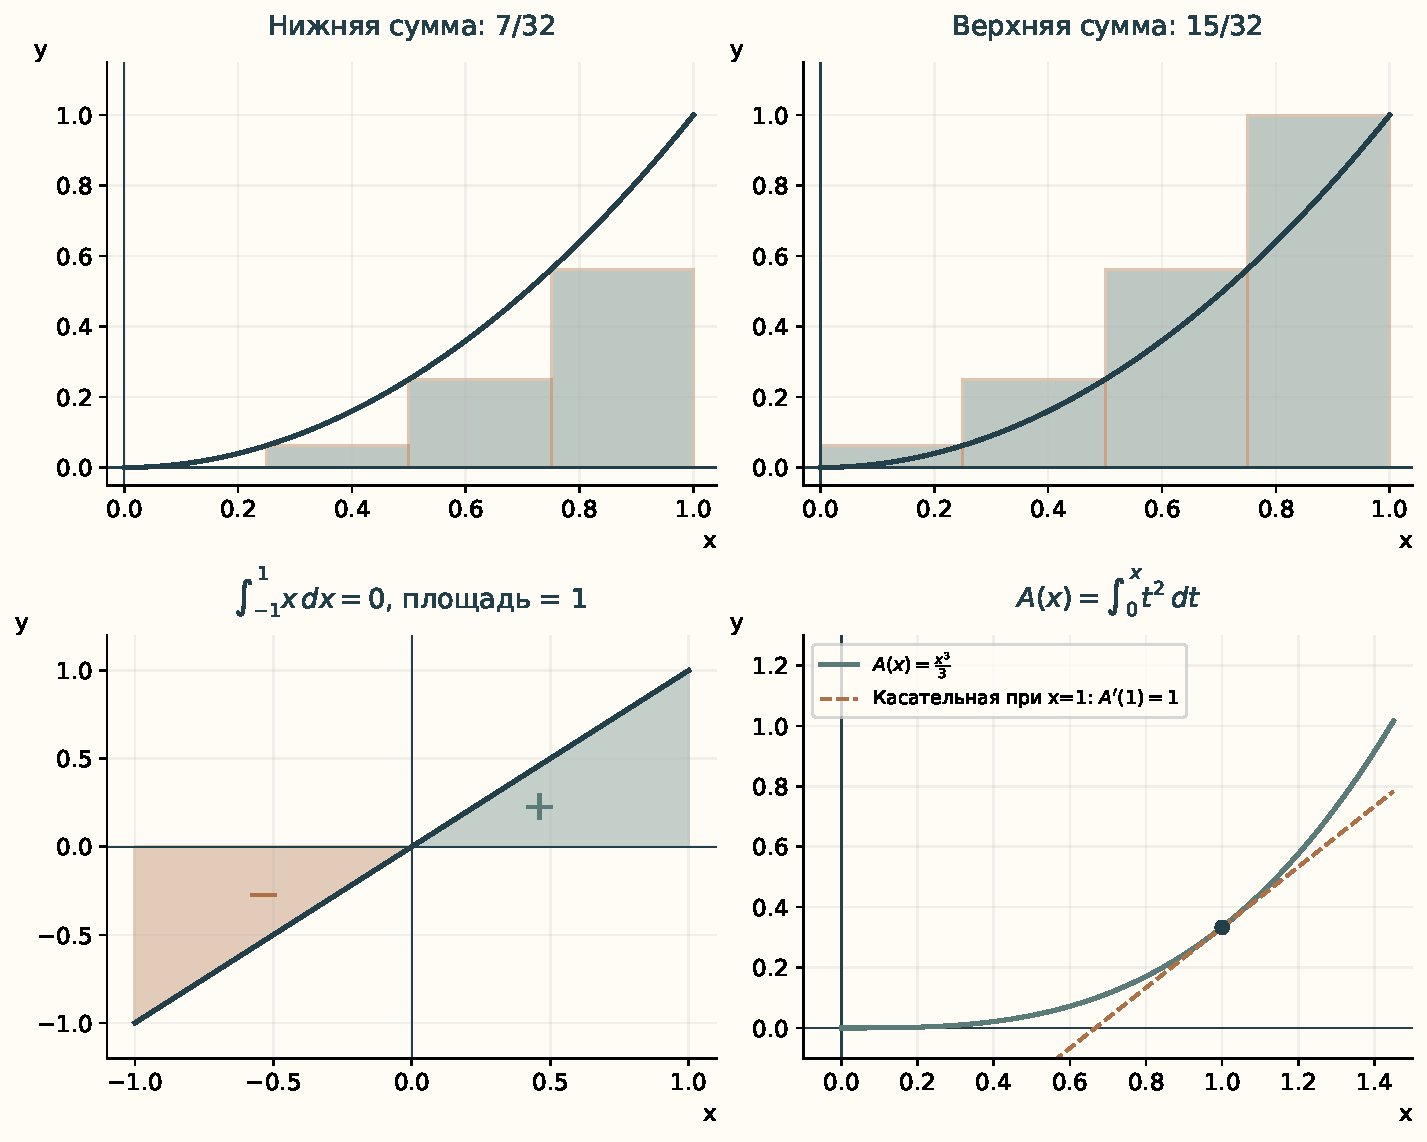
\includegraphics[width=\textwidth,height=.79\textheight,keepaspectratio]{images/atlas-integral.pdf}\par\small Суммы Дарбу и ориентированная площадь\end{center}\end{minipage}\par
\Needspace{7\baselineskip}\section*{Задачи}
\begingroup\setlength{\parskip}{2pt}
\noindent\begin{minipage}[t]{\linewidth}\textbf{41.1.} Для \(f(x)=x\) на \([0;2]\) и разбиения \(0,1,2\) найди нижнюю и верхнюю суммы Дарбу.\par\end{minipage}\par
\noindent\begin{minipage}[t]{\linewidth}\textbf{41.2.} Для \(f(x)=x^2\) на \([0;1]\) и четырёх равных частей вычисли суммы Дарбу и проверь, что \(\dfrac13\) лежит между ними.\par\end{minipage}\par
\noindent\begin{minipage}[t]{\linewidth}\textbf{41.3.} Вычисли \(\int_1^4 3\,dx\), \(\int_0^2 2x\,dx\), \(\int_{-1}^1 x\,dx\).\par\end{minipage}\par
\noindent\begin{minipage}[t]{\linewidth}\textbf{41.4.} Найди площадь между графиком \(y=x\) и осью \(x\) на \([-1;1]\). Сравни с интегралом функции.\par\end{minipage}\par
\noindent\begin{minipage}[t]{\linewidth}\textbf{41.5.} Вычисли \(\int_0^1(3x^2-2x+1)\,dx\).\par\end{minipage}\par
\par\addvspace{5pt}\begin{lrbox}{\CatFlowBox}\begin{minipage}[t]{\linewidth}
\setlength{\parskip}{5pt}\setlength{\columnsep}{4.5mm}\setlength{\intextsep}{0pt}
\begin{wrapfigure}[11]{r}{54mm}

\includegraphics[width=54mm,height=58mm,keepaspectratio]{images/unique/art-124.png}
\label{catflow:124}
\end{wrapfigure}
\textbf{41.6.} Найди \(\int_1^e\dfrac1x\,dx\) и \(\int_0^{\pi/2}\cos x\,dx\).\par

\textbf{41.7.} Известно, что \(\int_0^1 f=2\), \(\int_1^3 f=5\), \(\int_0^3 g=-1\). Найди \(\int_0^3(2f-g)\) и \(\int_3^0 f\).\par

\textbf{41.8.} Найди все первообразные \(f(x)=4x^3-2\) на \(\mathbb R\).\par

\textbf{41.9.} Найди первообразную \(f(x)=2x\), удовлетворяющую условию \(F(1)=5\).\par
\par\WFclear\end{minipage}\end{lrbox}%
\ifdim\dimexpr\ht\CatFlowBox+\dp\CatFlowBox\relax<64mm\dp\CatFlowBox=\dimexpr64mm-\ht\CatFlowBox\relax\fi%
\noindent\usebox{\CatFlowBox}\par\addvspace{5pt}

\noindent\begin{minipage}[t]{\linewidth}\textbf{41.10.} Проверь дифференцированием, что \(\int\operatorname{ch}x\,dx=\operatorname{sh}x+C\), и вычисли \(\int_0^{\ln2}\operatorname{ch}x\,dx\).\par\end{minipage}\par
\noindent\begin{minipage}[t]{\linewidth}\textbf{41.11.} Тележка движется по прямой со скоростью \(v(t)=2t+1\) м/с при \(0\le t\le3\) с. Найди перемещение за это время.\par\end{minipage}\par
\noindent\begin{minipage}[t]{\linewidth}\textbf{41.12.} Плотность тонкой рейки длины 2 м равна \(\rho(x)=1+x\) кг/м, где \(x\) отсчитывается от левого края в метрах. Найди массу.\par\end{minipage}\par
\noindent\begin{minipage}[t]{\linewidth}\textbf{41.13.} Среднее значение непрерывной функции на \([a;b]\) определяют как \(\dfrac1{b-a}\int_a^b f(x)\,dx\). Найди среднее значение \(f(x)=x^2\) на \([0;3]\).\par\end{minipage}\par
\noindent\begin{minipage}[t]{\linewidth}\textbf{41.14.} Для \(A(x)=\int_1^x(t^2+1)\,dt\) найди \(A'(x)\) и \(A(1)\).\par\end{minipage}\par
\noindent\begin{minipage}[t]{\linewidth}\textbf{41.15.} Вычисли заменой переменной \(\int_0^1 2x e^{x^2}\,dx\).\par\end{minipage}\par
\noindent\begin{minipage}[t]{\linewidth}\textbf{41.16.} Вычисли по частям \(\int_0^1 xe^x\,dx\).\par\end{minipage}\par
\noindent\begin{minipage}[t]{\linewidth}\textbf{41.17.} Применима ли формула \(\int_{-1}^1\dfrac1x\,dx=[\ln|x|]_{-1}^1=0\) в смысле введённого здесь интеграла Римана?\par\end{minipage}\par
\noindent\begin{minipage}[t]{\linewidth}\textbf{41.18.} Докажи оценку \(\left|\int_a^b f(x)\,dx\right|\le M(b-a)\), если \(a<b\), функция интегрируема и \(|f(x)|\le M\).\par\end{minipage}\par
\noindent\begin{minipage}[t]{\linewidth}\textbf{41.19.}\starmark{} Докажи, что непрерывная неотрицательная функция на невырожденном отрезке с нулевым интегралом тождественно равна нулю.\par\end{minipage}\par
\noindent\begin{minipage}[t]{\linewidth}\textbf{41.20.} Докажи: если \(F'=G'\) на интервале, то \(F-G\) постоянна на нём.\par\end{minipage}\par
\noindent\begin{minipage}[t]{\linewidth}\textbf{41.21.}\starmark{} Найди \(\dfrac{d}{dx}\int_0^{x^2}\cos t\,dt\) и объясни оба использованных правила.\par\end{minipage}\par
\noindent\begin{minipage}[t]{\linewidth}\textbf{41.22.}\starmark{} Вычисли \(\int_0^\pi \cos t\,e^{\sin t}\,dt\). Объясни, почему немонотонность \(\sin t\) не мешает формуле замены.\par\end{minipage}\par
\noindent\begin{minipage}[t]{\linewidth}\textbf{41.23.}\starmark{} Докажи формулу \(\int_0^b x\,dx=\dfrac{b^2}2\), \(b>0\), только через суммы Дарбу на \(n\) равных частях.\par\end{minipage}\par
\noindent\begin{minipage}[t]{\linewidth}\textbf{41.24.}\starmark{} Докажи теорему о среднем для интеграла: для непрерывной \(f\) на \([a;b]\), \(a<b\), существует \(c\in[a;b]\) с \(\int_a^b f(x)\,dx=f(c)(b-a)\).\par\end{minipage}\par
\noindent\begin{minipage}[t]{\linewidth}\textbf{41.25.} Вычисли \(\int_1^\infty\dfrac{dx}{x^3}\).\par\end{minipage}\par
\noindent\begin{minipage}[t]{\linewidth}\textbf{41.26.} Исследуй сходимость \(\int_1^\infty\dfrac{dx}{\sqrt x}\).\par\end{minipage}\par
\noindent\begin{minipage}[t]{\linewidth}\textbf{41.27.} Вычисли \(\int_0^1\dfrac{dx}{\sqrt x}\).\par\end{minipage}\par
\noindent\begin{minipage}[t]{\linewidth}\textbf{41.28.} Для \(\lambda>0\) вычисли \(\int_0^\infty e^{-\lambda x}\,dx\).\par\end{minipage}\par
\noindent\begin{minipage}[t]{\linewidth}\textbf{41.29.}\starmark{} Объясни, почему \(\int_{-1}^1\dfrac{dx}{x}\) не существует, хотя симметричные отсечения дают нуль.\par\end{minipage}\par
\noindent\begin{minipage}[t]{\linewidth}\textbf{41.30.} Вычисли \(\int_{-\infty}^{\infty}\dfrac{dx}{1+x^2}\), рассматривая обе половины отдельно.\par\end{minipage}\par
\noindent\begin{minipage}[t]{\linewidth}\textbf{41.31.} После изучения интеграла найди площадь между \(y=2x\) и \(y=x^2\).\par\end{minipage}\par
\noindent\begin{minipage}[t]{\linewidth}\textbf{41.32.} Найди все первообразные \(3x^2-2x+1\) на \(\mathbb R\), затем выбери ту, для которой \(F(0)=5\).\par\end{minipage}\par
\par\Needspace{12\baselineskip}\section*{Олимпиадные задачи}
\par\addvspace{2pt}\begin{lrbox}{\CatFlowBox}\begin{minipage}[t]{\linewidth}
\setlength{\parskip}{2pt}\setlength{\columnsep}{4.5mm}\setlength{\intextsep}{0pt}
\begin{wrapfigure}[10]{r}{54mm}

\includegraphics[width=54mm,height=58mm,keepaspectratio]{images/unique/art-320.png}
\label{catflow:320}
\end{wrapfigure}
\textbf{41.33.}\starmark{} {\small\itshape\href{https://www.imc-math.org.uk/imc1996/prob_sol.pdf}{IMC, 1996, день 1, № 2}; перевод.}\par Для натурального \(n\) вычисли \[I_n=\int_{-\pi}^{\pi}\dfrac{\sin(nx)}{(1+2^x)\sin x}\,dx.\] В точках \(x=0,\pm\pi\) подынтегральная функция доопределяется по непрерывности.\par

\textbf{41.34.}\starmark{} {\small\itshape\href{https://www.imc-math.org.uk/imc1998/prob_sol1.pdf}{IMC, 1998, день 1, № 6}; перевод.}\par Непрерывная \(f:[0,1]\to\mathbb R\) удовлетворяет \(xf(y)+yf(x)\le1\) при любых \(x,y\in[0,1]\). Докажи \(\int_0^1 f(x)\,dx\le\dfrac\pi4\) и найди функцию, достигающую равенства.\par

\textbf{41.35.}\starmark{} {\small\itshape\href{https://www.imc-math.org.uk/imc1995/prob_sol.pdf}{IMC, 1995, день 1, № 4}; перевод.}\par Докажи инъективность функции \(F(x)=\int_x^{x^2}\dfrac{dt}{\ln t}\), \(x>1\), и найди множество её значений.\par
\par\WFclear\end{minipage}\end{lrbox}%
\ifdim\dimexpr\ht\CatFlowBox+\dp\CatFlowBox\relax<58mm\dp\CatFlowBox=\dimexpr58mm-\ht\CatFlowBox\relax\fi%
\noindent\usebox{\CatFlowBox}\par\addvspace{2pt}

\endgroup
